\documentclass{beamer}

\usepackage[utf8]{inputenc}
\usepackage{default}
\usepackage{amsmath}

\title{A Tutorial on Multigrid Methods}
\author{Philip Greggory Lee}
\institute{
 Electrical Engineering and Computer Science\\
 Northwestern University\\
 Evanston, IL 60208
}

\AtBeginSection
{
 \begin{frame}{Outline}
  \tableofcontents[currentsection]
 \end{frame}
 \addtocounter{framenumber}{-1}
}

\providecommand{\defeq}{\stackrel{\Delta}{=}}

\begin{document}

\begin{frame}
 \titlepage
\end{frame}

\begin{frame}{Outline}
 \tableofcontents
\end{frame}
\addtocounter{framenumber}{-1}

\section{Introduction}%========================================================

\begin{frame}{The Problem}
 \begin{itemize}
  \item Suppose we have a linear system whose variable $u$ represents a discretization
        of a function $g(x)$ on a regular grid.
  \begin{align}
   Au=f
  \end{align}
  \item As the level of discretization grows, so does the size of the system.
  \item In many typical cases, the condition number of $A$ grows with the
        square of the size of $u$.
  \item Simple linear solvers therefore slow down dramatically as the resolution
        increases.
 \end{itemize}
\end{frame}

\begin{frame}{The Intuition}
 \begin{itemize}
  \item Why should this be the case?
  \item In most cases, increasing the resolution does not \textit{really}
        introduce more complexity into the problem.
  \item Is there any way we can take advantage of the notion of
        \textit{resolution} of the solution $u$ in a principled way?
  \item The answer is yes, and we will explore a class of ways to do so called
        \textbf{multigrid methods}.
 \end{itemize}
\end{frame}

\begin{frame}[allowpagebreaks]{Notation}
 
\end{frame}

\section{The Motivating Example}%==============================================

\begin{frame}[allowframebreaks]{1D Laplace Problem}
 \begin{itemize}
  \item A simple example that serves to illustrate the major points of this
        tutorial is the Laplace equation in 1D.
  \begin{align}
   -\Delta u = -\nabla \cdot \nabla u = 0
  \end{align}
  \item In this case, the Laplace operator $\Delta$ can be represented by
        convolution with the kernel $[1,-2,1] = [1,-1]\ast[1,-1]$.
  \begin{figure}
   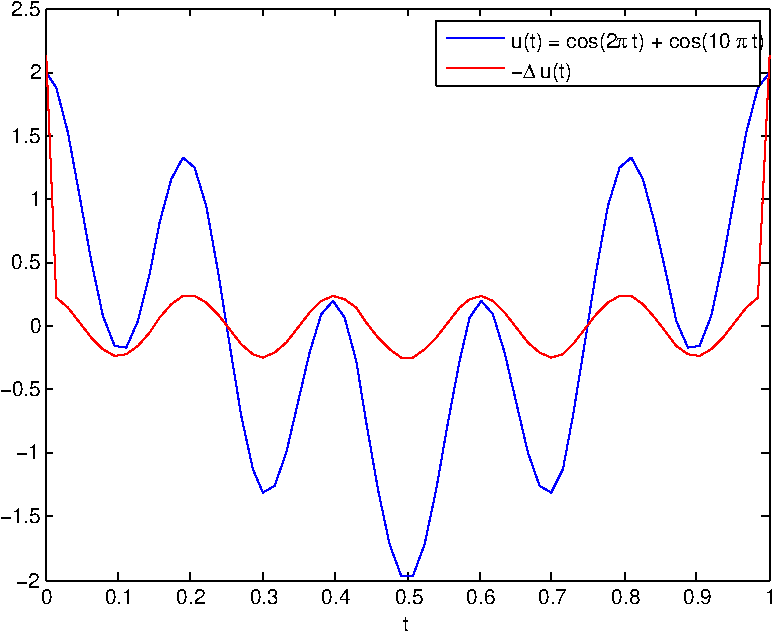
\includegraphics[width=6cm]{images/laplaceOperatorExample.pdf}
  \end{figure}
  \item 
 \end{itemize}
\end{frame}


\section{Relaxation (Iterative Methods)}%======================================

\section{Nested Iteration}%====================================================

\section{Basic Multigrid Methods}%=============================================

\section{Analysis}%============================================================

\section{Recent Work}%=========================================================

% References ==================================================================
\begin{frame}[allowframebreaks]
 \frametitle{References}
 \bibliographystyle{amsalpha}
 \bibliography{multigridrefs.bib}
\end{frame}

\end{document}
